
%-------------------------------------------------------------------------------------
\section[A first evaluation of LES with in-situ \& remote observations]{A first evaluation of LES with in-situ \& remote observations}
\label{sectionCampagne}

The pertinence and the accuracy of the high-resolution Large Eddy Simulations performed so far crucially need to be evaluated based on in-situ or remote observations of both the regional and fine scales of the real ocean. The observation of the latter is somehow difficult at least when these fine scales are localized in small, transient spots. In turn, LES can then appear as a well-adapted tool to help designing the campaign.

In the present section, only a selection of in-situ and remote observations of Gibraltar 2020 campaign is studied. While the exploitation of campaign data is incomplete, some observations are still presented to represent the complete work that was carried out during my Ph-D to provide an as-rigorous-as-possible work including both development of LES, investigation of LES dynamics and evaluation with dedicated observations. Further treatment of in-situ observations and the preparation of the Gibraltar 2022 campaign are still being carried out.

\subsection{Field campaign Gibraltar 2020 (an overview)}
The field campaign of in situ measurements Gibraltar 2020 has been carried out by SHOM during the fall of 2020 in the Strait of Gibraltar and in the western part of the Alboran sea aboard the research and survey ship \textit{L'Atalante}. This campaign and the following Gibraltar 2022 campaign are part of the PrometeVs program and LEFE-GEPETO project. On-site measures were taken by ship-based instruments from 8/10/2020 to 20/10/2020. Among those, sampling of the water column at both end of the strait were realized; at the eastern end of the strait on the 14th and 15th October, and at its western end on the 16th of October.

Additionally, five moorings were deployed as presented in Table \noparref{tab_moor}, locations are also indicated in Figure \noparref{fig_moor}.A2. Mooring Mo1 is positioned west of the slope of Camarinal Sill. Mooring Mo3 is placed in the southern deep half of CS whereas Mo2 is positioned in a shallow area at the center. Mo4 and Mo5 are positioned near each other at some distance east of CS. Three of the moorings (Mo1, Mo3 and Mo5) are equipped with CTD sensors to provide hydrological characteristics of the water masses, and the other two (Mo2 and Mo4) with ADCP sensors to sample the currents in the water column. Sampling frequencies range from a few tens of seconds to one minute.

\begin{table}[!h]
        \centering
        \begin{tabular}{|c|c|c|c|}
                \hline
                Mooring & type & position & date (UTC)\\ 
                 \hline
                Mo1 & CTD & 35° 55.264'N ; 5° 46.739'W & 8/10/2020 15h - 9/11/2020 12h\\
                Mo2 & ADCP & 35° 55.761'N ; 5° 45.288'W & 8/10/2020 5h - 17/10/2020 15h\\
                Mo3 & CTD & 35° 54.719'N ; 5° 44.459'W & 8/10/2020 13h - 22/10/2020 21h\\
                Mo4 & ADCP & 35° 55.870'N ; 5° 41.020'W & 8/10/2020 7h - 17/10/2020 14h\\
                Mo5 & CTP & 35° 56.229'N ; 5° 41.026'W & 8/10/2020 9h - 1/11/2020 14h\\
                \hline
        \end{tabular}
        \captionof{table}{Name, type of sensors, coordinates and date of deployment for moorings during Gibraltar 2020 field campaign.}
        \label{tab_moor}
        %\end{minipage}
\end{table}
In Section \noparref{section_obs_moor}, mooring data from Mo2, Mo4 and Mo5 are analyzed for a first observation period covering the ten-day period 8/10 to 18/10 during which, as indicated in Table \noparref{tab_moor}, both types of moorings data are available.


\subsection{Insights from LES simulations in preparation of Gibraltar 2020}

The numerical simulations presented in Section \noparref{sectionSim3D} are based on a high-resolution, non-hydrostatic model. Atmospheric fluxes are neglected as a first step toward realistic, high- resolution Large Eddy Simulation of the region of Gibraltar strait. This simulations provide information on the flow and processes occurring in the strait that were used to design the Gibraltar 2020 campaign.

 
\begin{figure}[!h]
 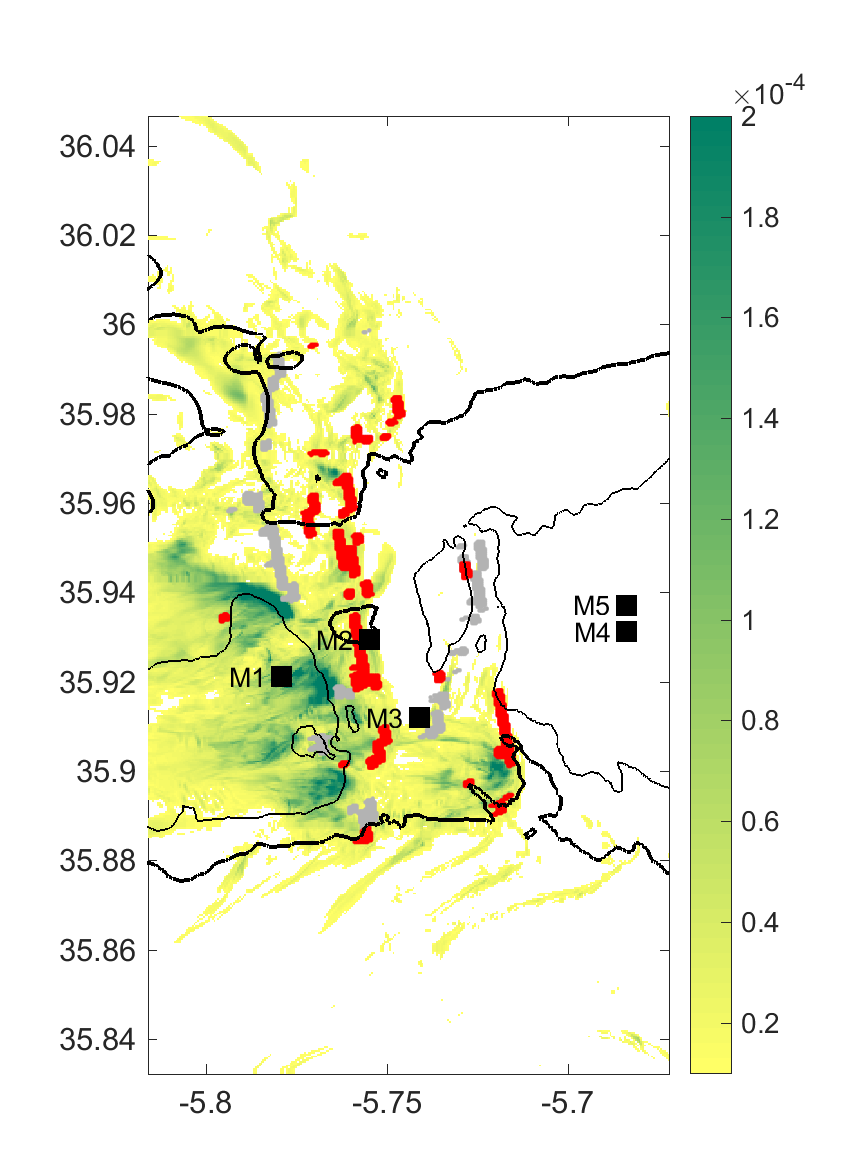
\includegraphics[width=\textwidth]{./GBR3D/Fig_Moor.png}
 \caption [(A)Locations of moorings and water column sampling stations. (B) $\Theta$-S diagrams.]{(A1) Water column sampling sites for (B1) and (B2). (A2) locations of moorings deployed during Gibraltar 2020 (black squares), over the map of standard deviations of parameter Q (colorbar) and the location of the hydraulic jumps of w-type and s-type from high-resolution numerical modelling of the strait of Gibraltar, as presented in Section \noparref{sectionSim3D}. (B1 and B2) $\Theta$-S diagrams for the series of water column sampling carried out respectively at the western and eastern exit of the Strait, water mass definitions according to \citet{Naranjo2015}.}
 \label{fig_moor}
\end{figure}

The field of standard deviation of parameter Q and the localization of the hydraulic jumps in figure (\noparref{fig_moor}.b) are for instance issued from those simulations. In combination with external restrictions such as the dense maritime traffic, strong currents and steep slopes of the area, such diagnosis and others were studied to chose the mooring deployment as well as the transect plans for the campaign (not shown). As an example, Mo1 was positioned down the western slope of the sill, i.e. down-flow of a potential primary instability generation area (see Sections \noparref{PartDiag3D} and \noparref{section3DResFlow} for a discussion of this diagnosis in high-resolution numerical simulation).

Figure \noparref{fig_SARIES} features a comparison between a SAR image (figure (A)) of the strait of Gibraltar with the surface signature of a propagating ISW just east of CS, and the corresponding field of norm of the gradient of surface currents in SimIT at the same date (figure (B)), showing a traveling wave in the same vicinity. Whereas the shape of the train itself differs in the model and observed fields, the simulation gives an accurate idea of the propagation speed of ISWs in the strait of Gibraltar. This was used to predict the position of ISW in relation to the tidal cycle as predicted by the Spanish institute Puertos del Estado\footnote{http://www.puertos.es/}. The anticipation of position of ISWs train was accurate at least in the strait of Gibraltar itself. In the Alboran Sea, where the influence of the gyre on the form of the wave packet is important, prediction was not as accurate, with time of arrival being greatly delayed compared to our predictions. 

Beyond the propagation speed, the high resolution of the model means that the shape of individual solitary waves is accurate as it propagates. This is used in the following Section \noparref{section_obs_moor} to help in the interpretation of mooring data from Mo4 and Mo5.

\begin{figure}[!h]
% \centering
 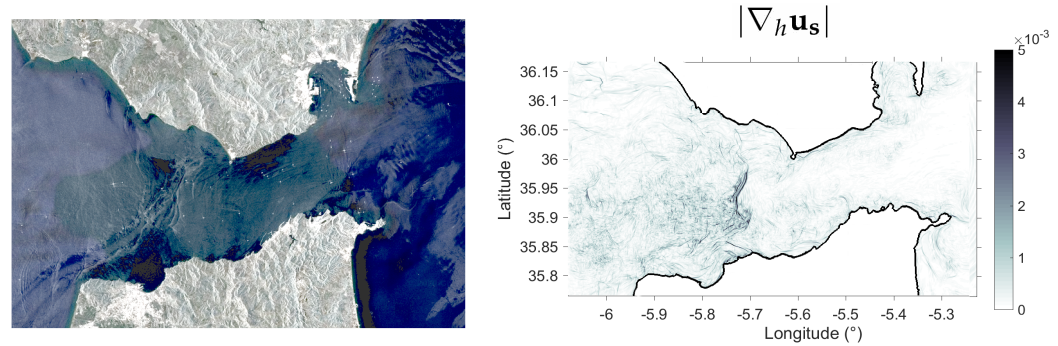
\includegraphics[width=\textwidth]{./GBR3D/Comp_SAR_IES.png}
 \caption[(A) Sentinel-1 SAR image. (B) Norm of the gradient of surface horizontal velocity in SimIT.] {(a) Sentinel-1 Synthetic Aperture Radar (SAR) image (12/09/2017 - 6h18pm UTC). (b) Norm of the gradient of surface horizontal velocity ($s^{-1}$) in the simulation SimIT (12/09/2017 - 6h30pm or t = 35h30 in simulation time) presented in Section \noparref{sectionSim3D}.}
 \label{fig_SARIES}
\end{figure}

\subsection{Overview of the mesoscale circulation during the observation period}

The in-situ time period covers one (for ship-based instruments and ADCP moorings) or two (for CTD moorings) neap-spring tide cycles. Figure \noparref{fig_moor_US3}.B shows the depth-averaged zonal component of the current measured at CS (data from Mo2 mooring). The measures begin during the neap-tide part of the fortnightly cycle. The west Alboran Gyre was also present in the West Alboran Sea during the field campaign (not shown). 

Figures \noparref{fig_moor}.B1 and B2 present the $\theta-S$ diagrams from ship-based water column sampling. For both figures, each color refers to a different sampling station indicated in Figure \noparref{fig_moor}.A1.

On the west end of the strait (Figure B1), no Mediterranean water was sampled at the southernmost station and a well-mixed signal could be identified at the northernmost station, delimiting the path of the Mediterranean outflow between 35.7$^{\text{o}}$ and 36$^{\text{o}}$ N. Among the signals of Mediterranean outflow waters, the two northernmost stations that reach depths shallower than 400 m (orange and yellow) show an enhanced mixing with NACW.

On the east end of the Strait (figure (B2)), WMDW can be found at depth for all stations except the northernmost (yellow). For the next two stations south of the latter, as well as the two southernmost stations, WMDW is mixed with intermediate waters. 

The five northernmost stations' surface waters are fresher waters than the SAW signal at the rest of the stations. This could be due to the northern stations being affected by the upwelling from the Iberian coast. The intermediate Mediterranean waters sampled at these stations are also warmer and saltier compared to the signal of the remaining four, which is interpreted as LIW.


\subsection{Solitary waves at Mo4 and Mo5 mooring and currents over CS at Mo2 mooring}
\label{section_obs_moor}

\begin{figure}[!h]
% \centering
 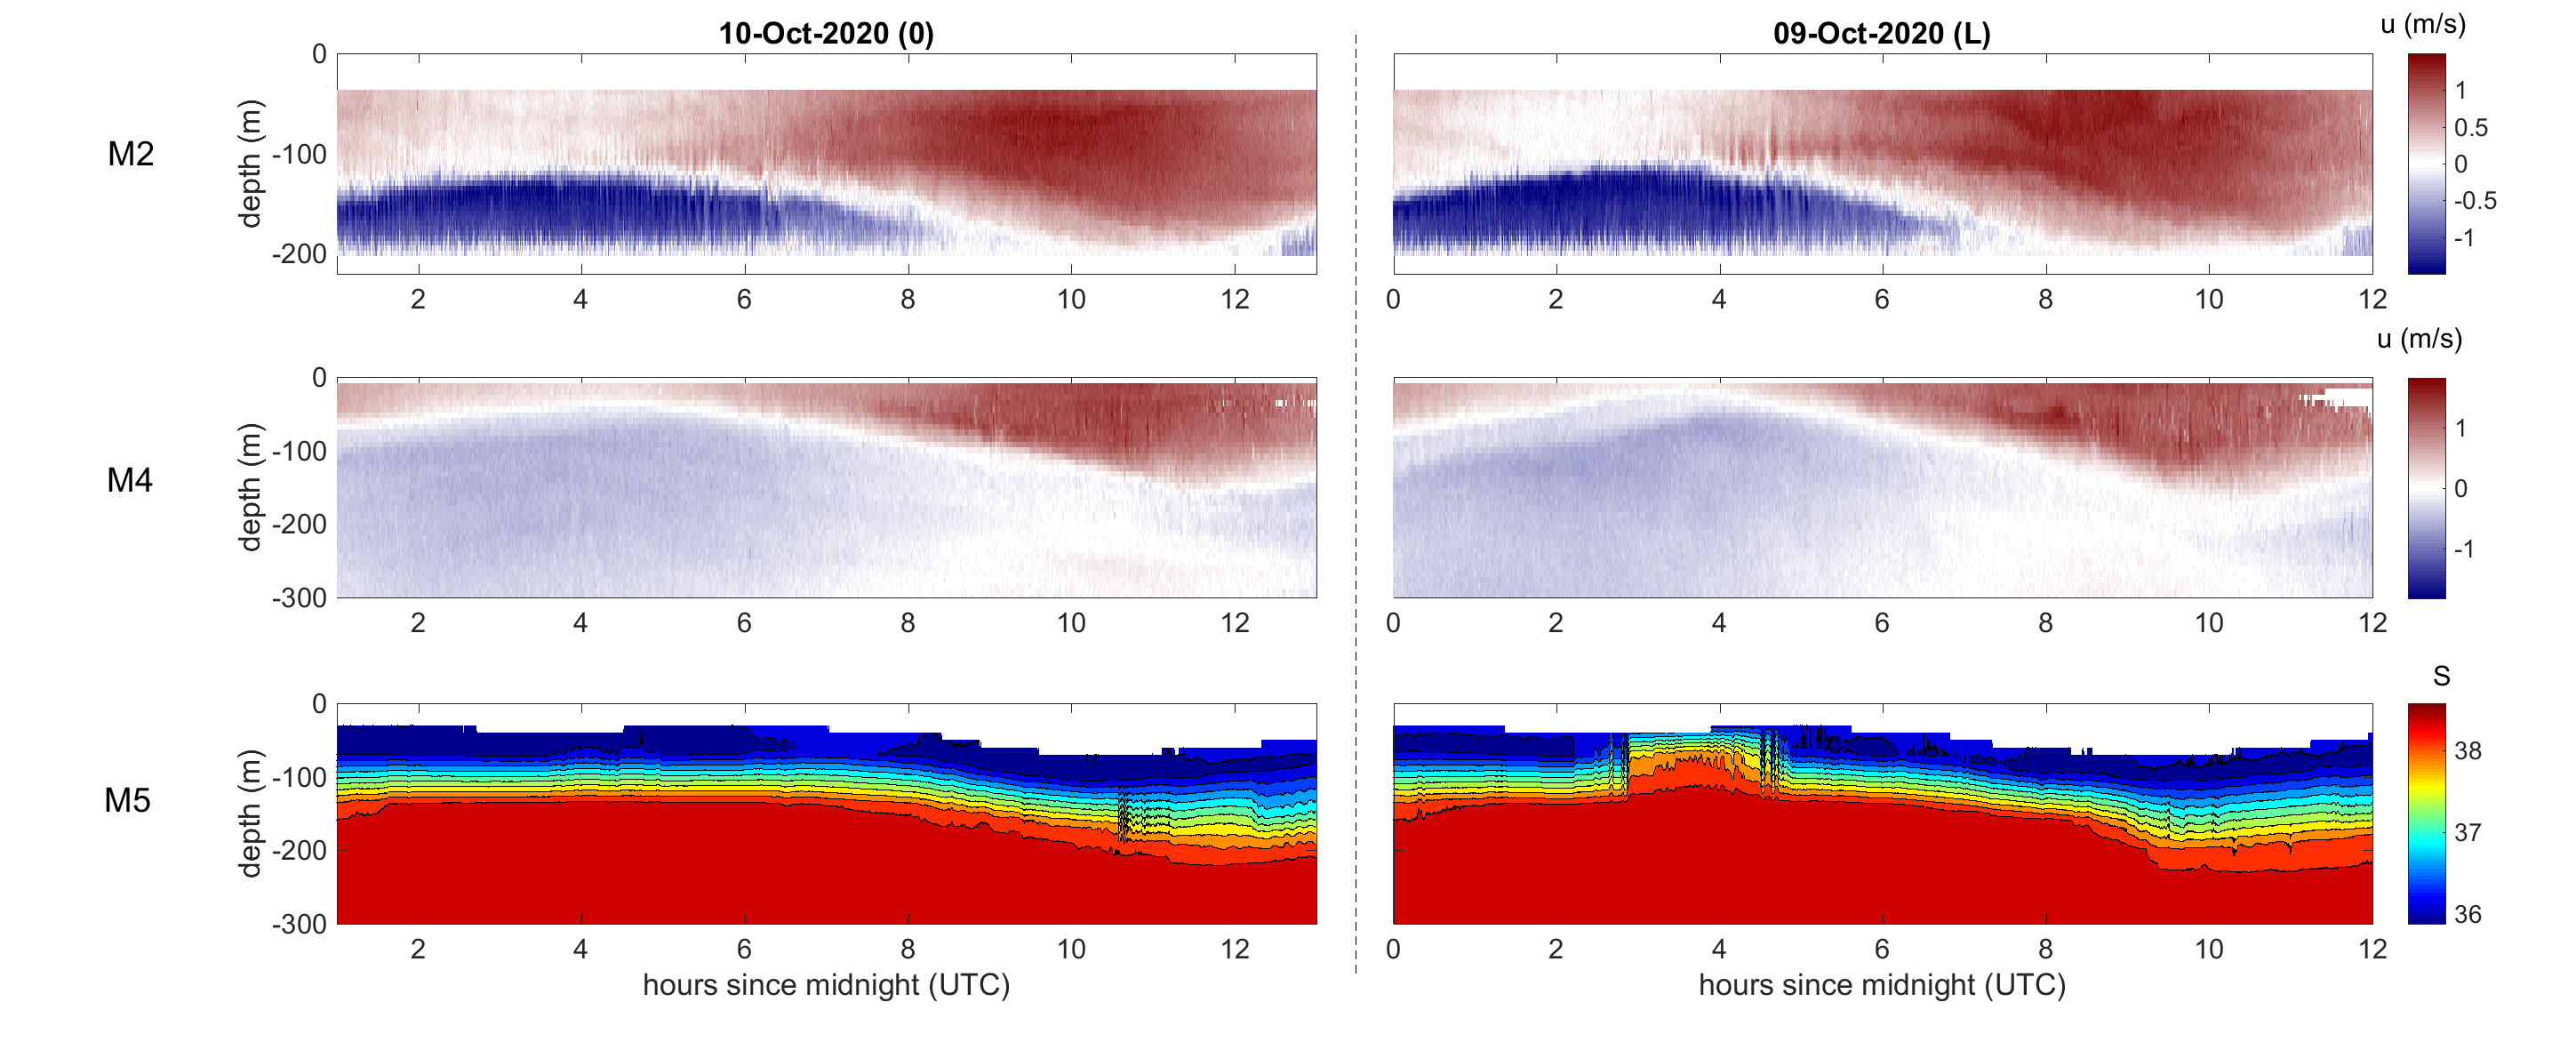
\includegraphics[width=\textwidth]{./GBR3D/US_moorings1.png}
 \caption [Time-series of mooring data from Mo2, Mo4 and Mo5]{Time-series of mooring data over the water column from Mo2 (upper row), Mo4 (center row) and Mo5 (lower row) mooring. The zonal component of currents is represented for Mo2 and Mo4 mooring, and the measured salinity at Mo5 mooring.}
 \label{fig_moor_US1}
\end{figure}

\begin{figure}[!h]
% \centering
 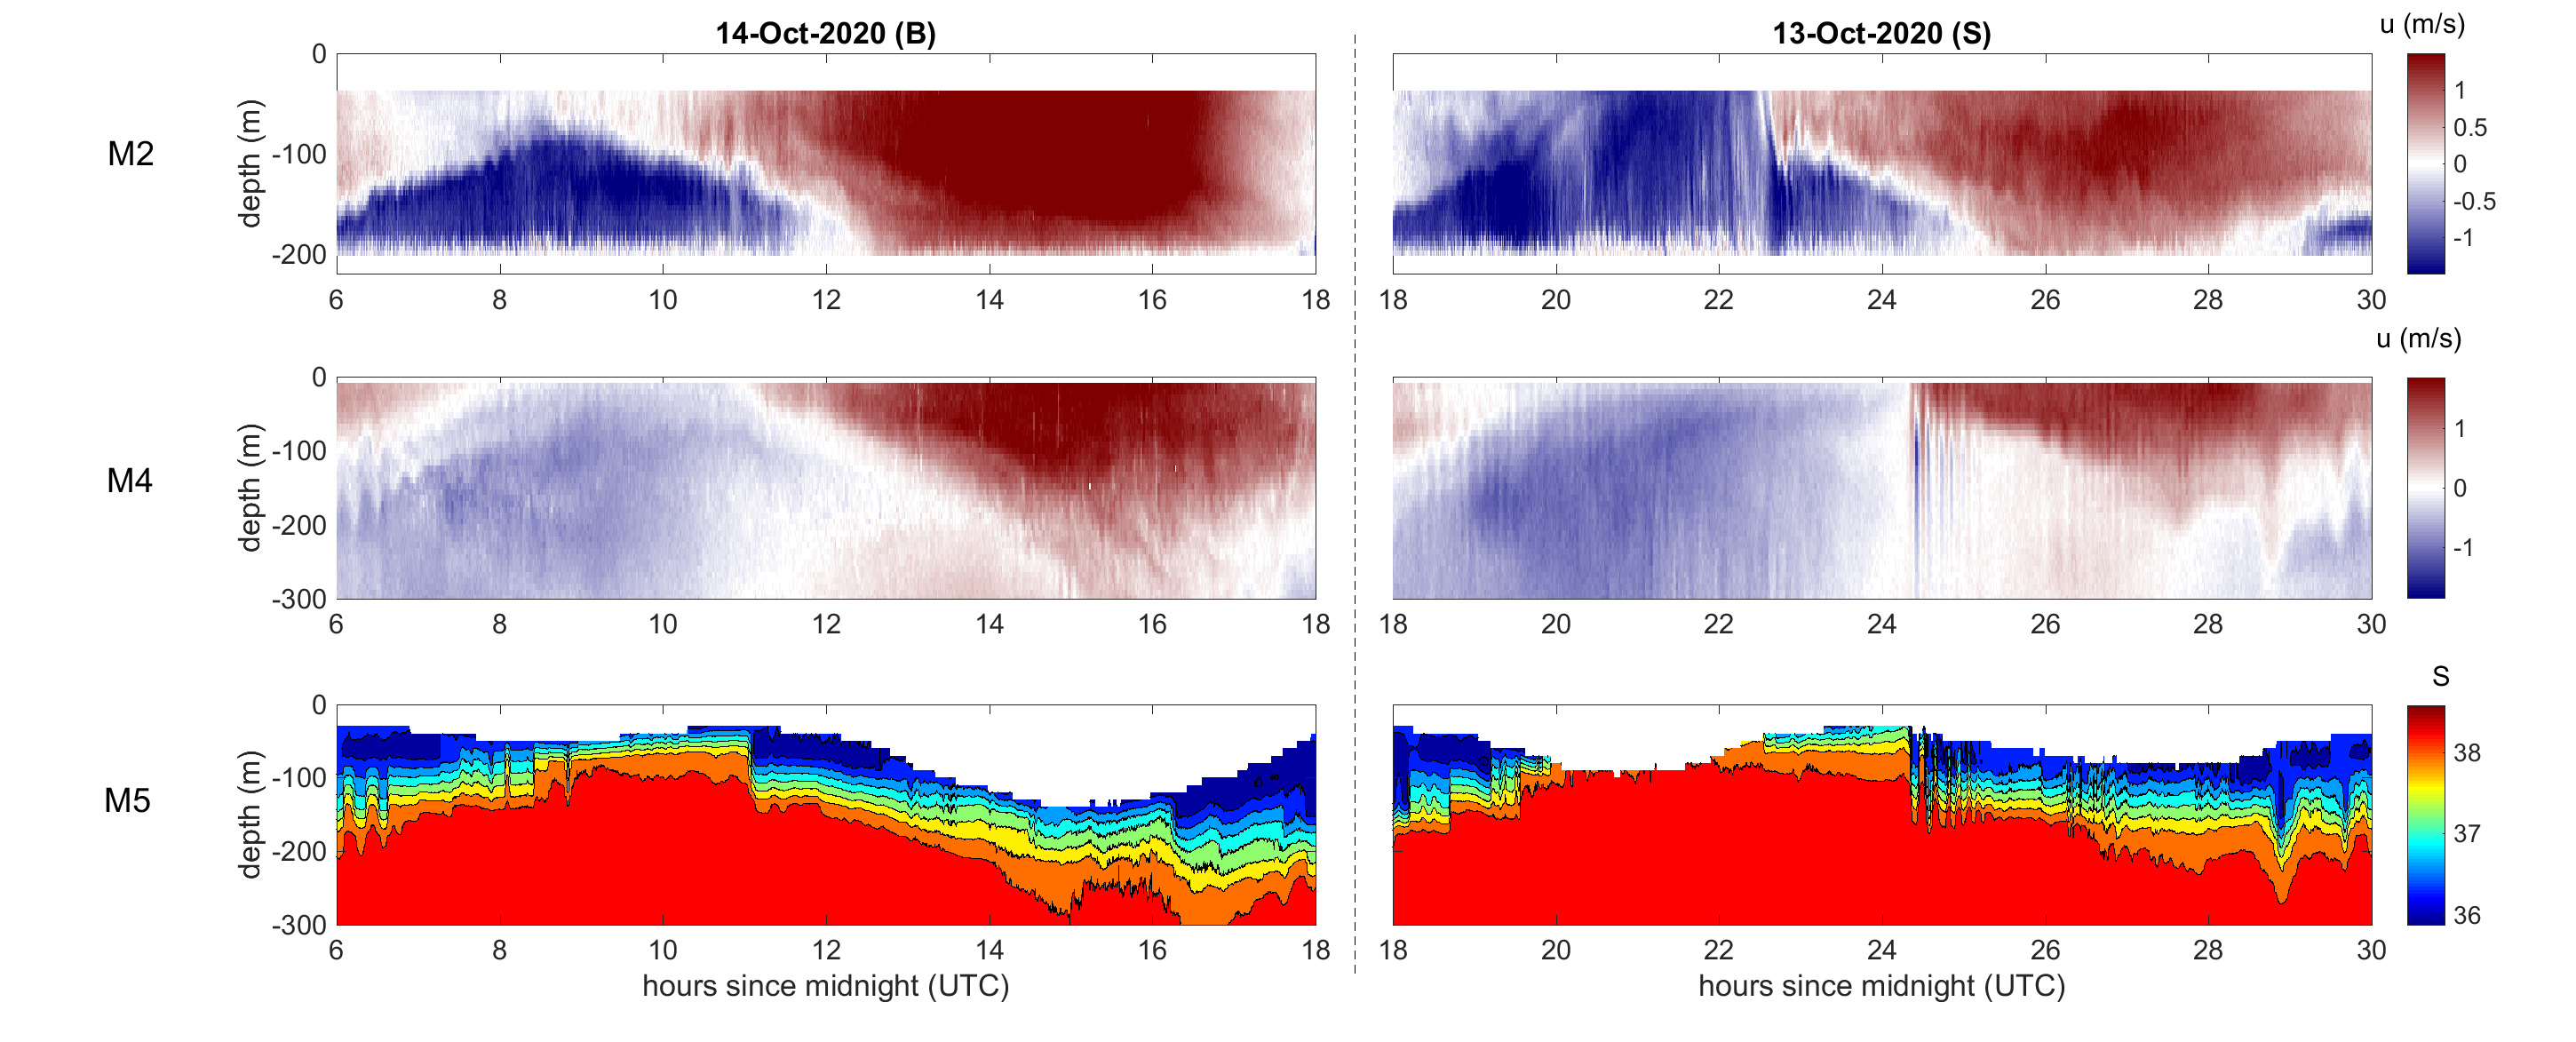
\includegraphics[width=\textwidth]{./GBR3D/US_moorings2.png}
 \caption [Time-series of mooring data from Mo2, Mo4 and Mo5]{same as Figure \noparref{fig_moor_US1} for different time-periods.}
 \label{fig_moor_US2}
\end{figure}

\begin{figure}[!h]
% \centering
 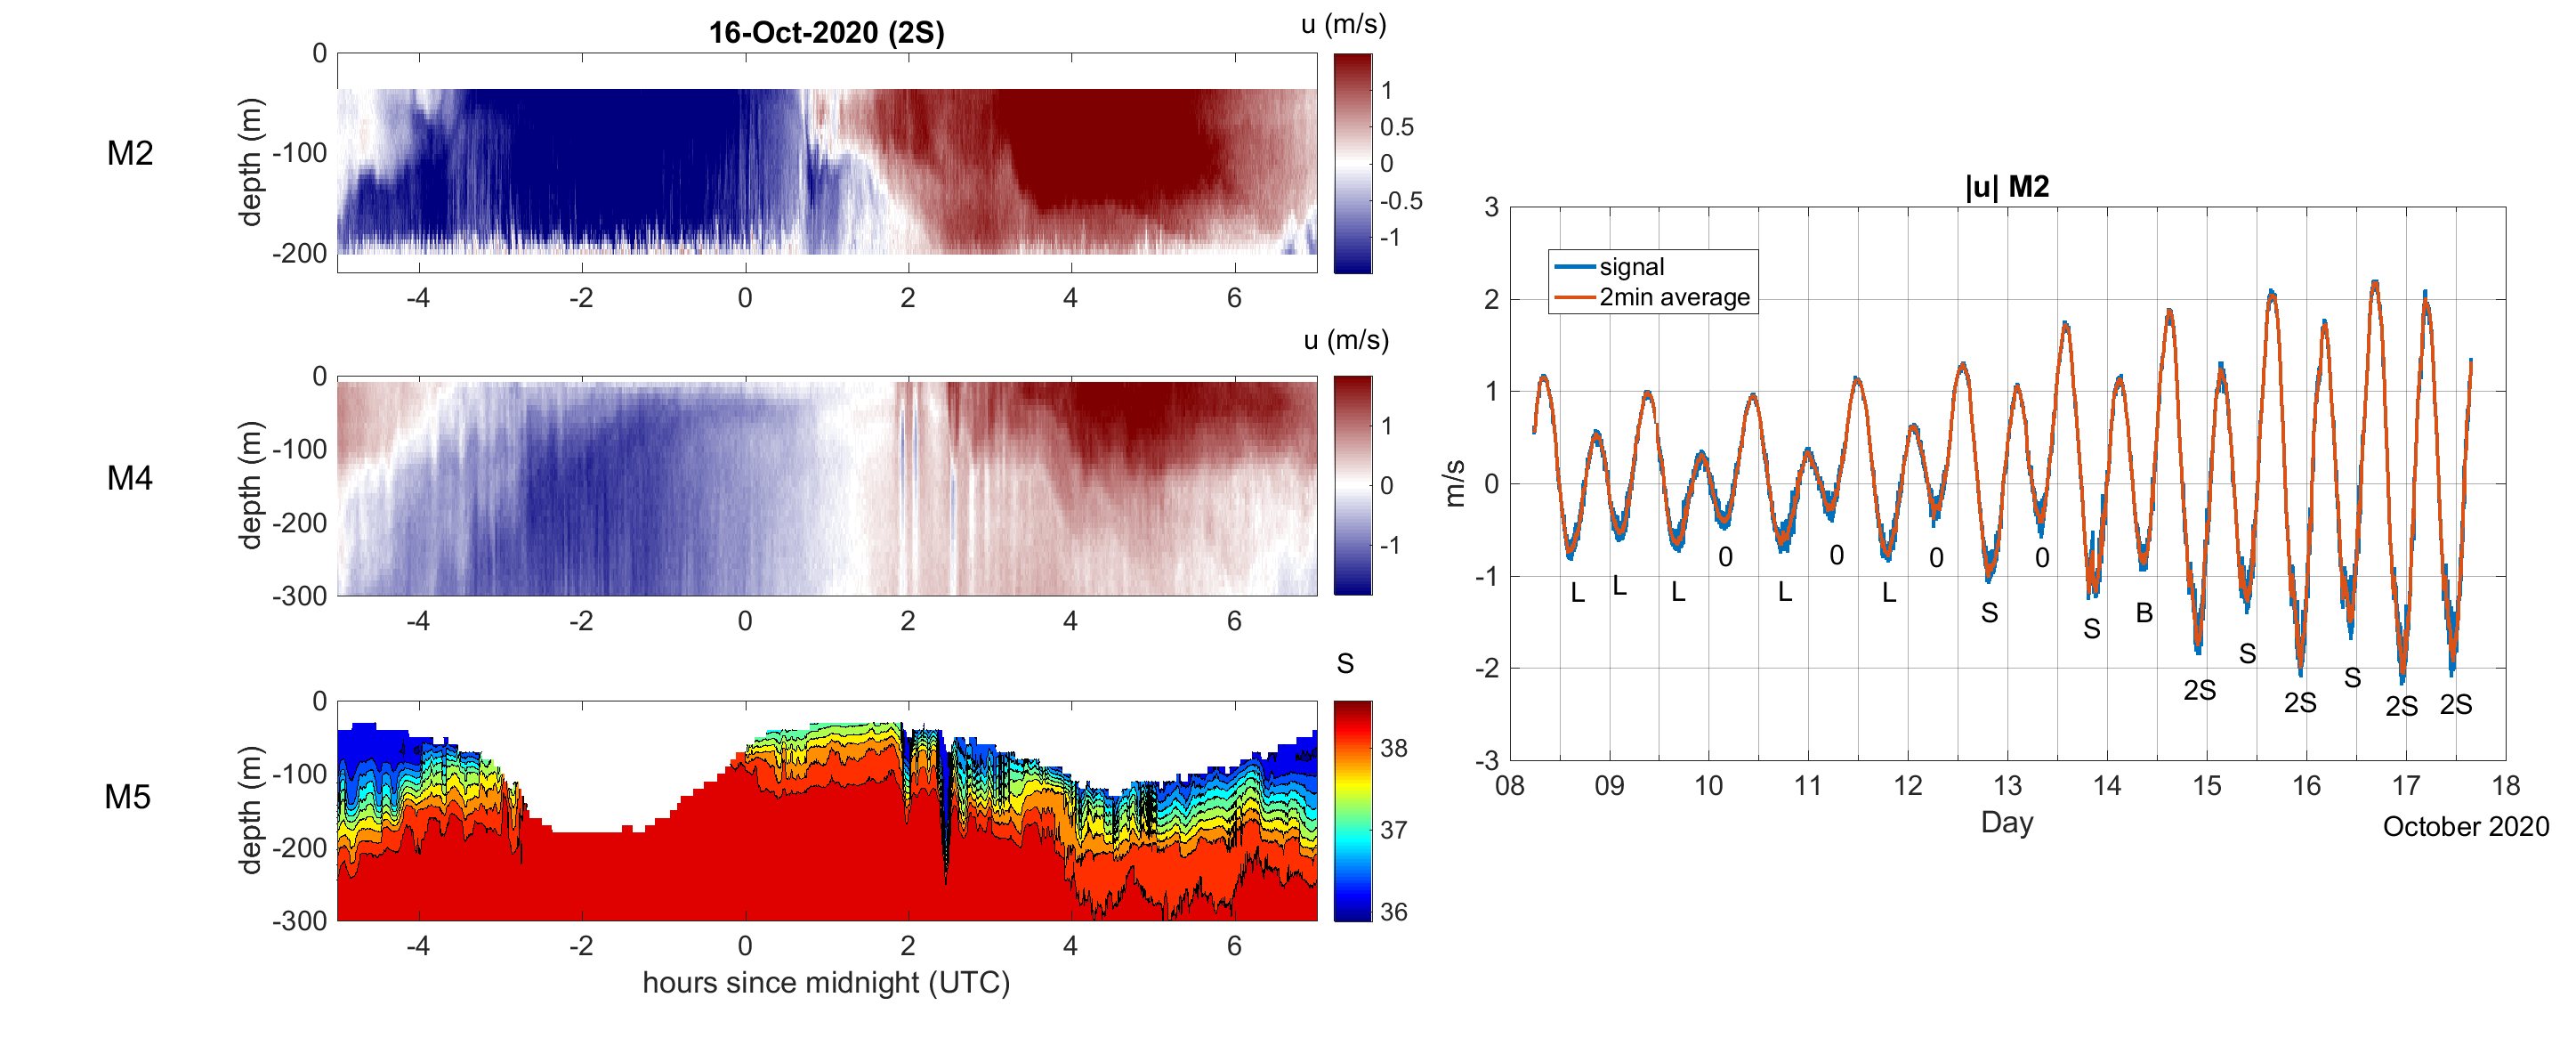
\includegraphics[width=\textwidth]{./GBR3D/US_moorings3.png}
 \caption [(A)Time-series of mooring data from Mo2, Mo4 and Mo5. (B) Depth-averaged signal of the zonal component of currents at Mo2 with type of signal observed at Mo4 and Mo5 after each outflow.]{(A1 to A3) Same as Figure \noparref{fig_moor_US1} but for a different time-period. (B) Time-series of depth-averaged signal of the zonal component of currents from Mo2 data (in blue the instant signal recorded, in red the 2 minutes average). For each outflow is indicated the type of signal that is observed at Mo4 and Mo5 mooring (see text).}
 \label{fig_moor_US3}
\end{figure}

Figures \noparref{fig_moor_US1} to \noparref{fig_moor_US3}.a present depth-time records of the zonal velocity (for Mo2 and Mo4 mooring) and salinity (for Mo5 mooring) for five different M2 tidal periods. Tilting by the strong currents provoked the depths of the CTD sensors of the Mo5 mooring to change overtime, sometime loosing the signal from tens to a hundred of meters at the top of the water column (for example see Figure \noparref{fig_moor_US2}.A3 at 15hUTC). Additionnally, note that whereas the whole water column is presented in those figures for the Mo2 data, only the upper 300 m (of a 500-m-deep water column) are represented here for Mo4 and Mo5 data for a better visualization.

Similarly, Figure \noparref{Fig_moor_USs} presents the zonal velocity and salinity of the upper 300 m of simulated data at a grid point of coordinate (35.937°N;5.706°W), near Mo4 and Mo5, from the simulations SimNT (Figures \noparref{Fig_moor_USs}.A and B), SimIT (C) and SimST (D) of Section \noparref{sectionSim3D}. Although those simulations cover a different time-period, the simulated fields present similar patterns of internal waves traveling in the water column as the observed data.


\subsubsection{Currents at Mo2 and Mo4 moorings}

In the observations of currents made at mooring Mo2, periods of inflows and outflows can be distinguished respectively as having mostly eastward or westward components over the water column. During inflow periods, there are always at least two hours during which the whole flow measured by the captors is eastward (for example between 10 and 12 hours in Figure \noparref{fig_moor_US1}.A1). During outflows, the current can be westward at all captors, as is the case in Figures \noparref{fig_moor_US2}.B1 and \noparref{fig_moor_US3}.A1, but this is not necessarily the case. 

In Figures \noparref{fig_moor_US1}.A1 and B1, for example, the baroclinic exchange structure of currents is still distinctive during outflows, with a weak eastward flow in the upper 120 m of the water column over a strong westward current. Figure \noparref{fig_moor_US2}.A1 presents another case for which the flow in the upper water column becomes momentarily weakly westward between t = 7 h and t = 9 h, with a still clear shear interface at 100-m deep.

In the numerical simulations performed in Section \noparref{sectionSim3D}, an entirely westward flowing water column at Mo2 mooring corresponds to an area a hydraulic jump is present. In Figure \noparref{fig_moor}.A2, this location corresponds to the upflow area of the two types of hydraulic jumps identified in Section \noparref{sectionSim3D} (s-jump and w-jump), and depicted respectively as grey and black points.

At mooring Mo4, the flow of the water column can become unidirectional during both outflow and inflow periods during the spring tide part of the fortnightly cycle. In this occasions, a shear area still subsists that matches with the salinity interface between Mediterranean and Atlantic waters identified at mooring Mo5 (see for example at t = 14 h in Figure \noparref{fig_moor_US2}.A2 and A3 at depth ranging between 150 and 200 m).

\subsubsection{Propagation of high frequency waves}

\begin{figure}[!h]
% \centering
 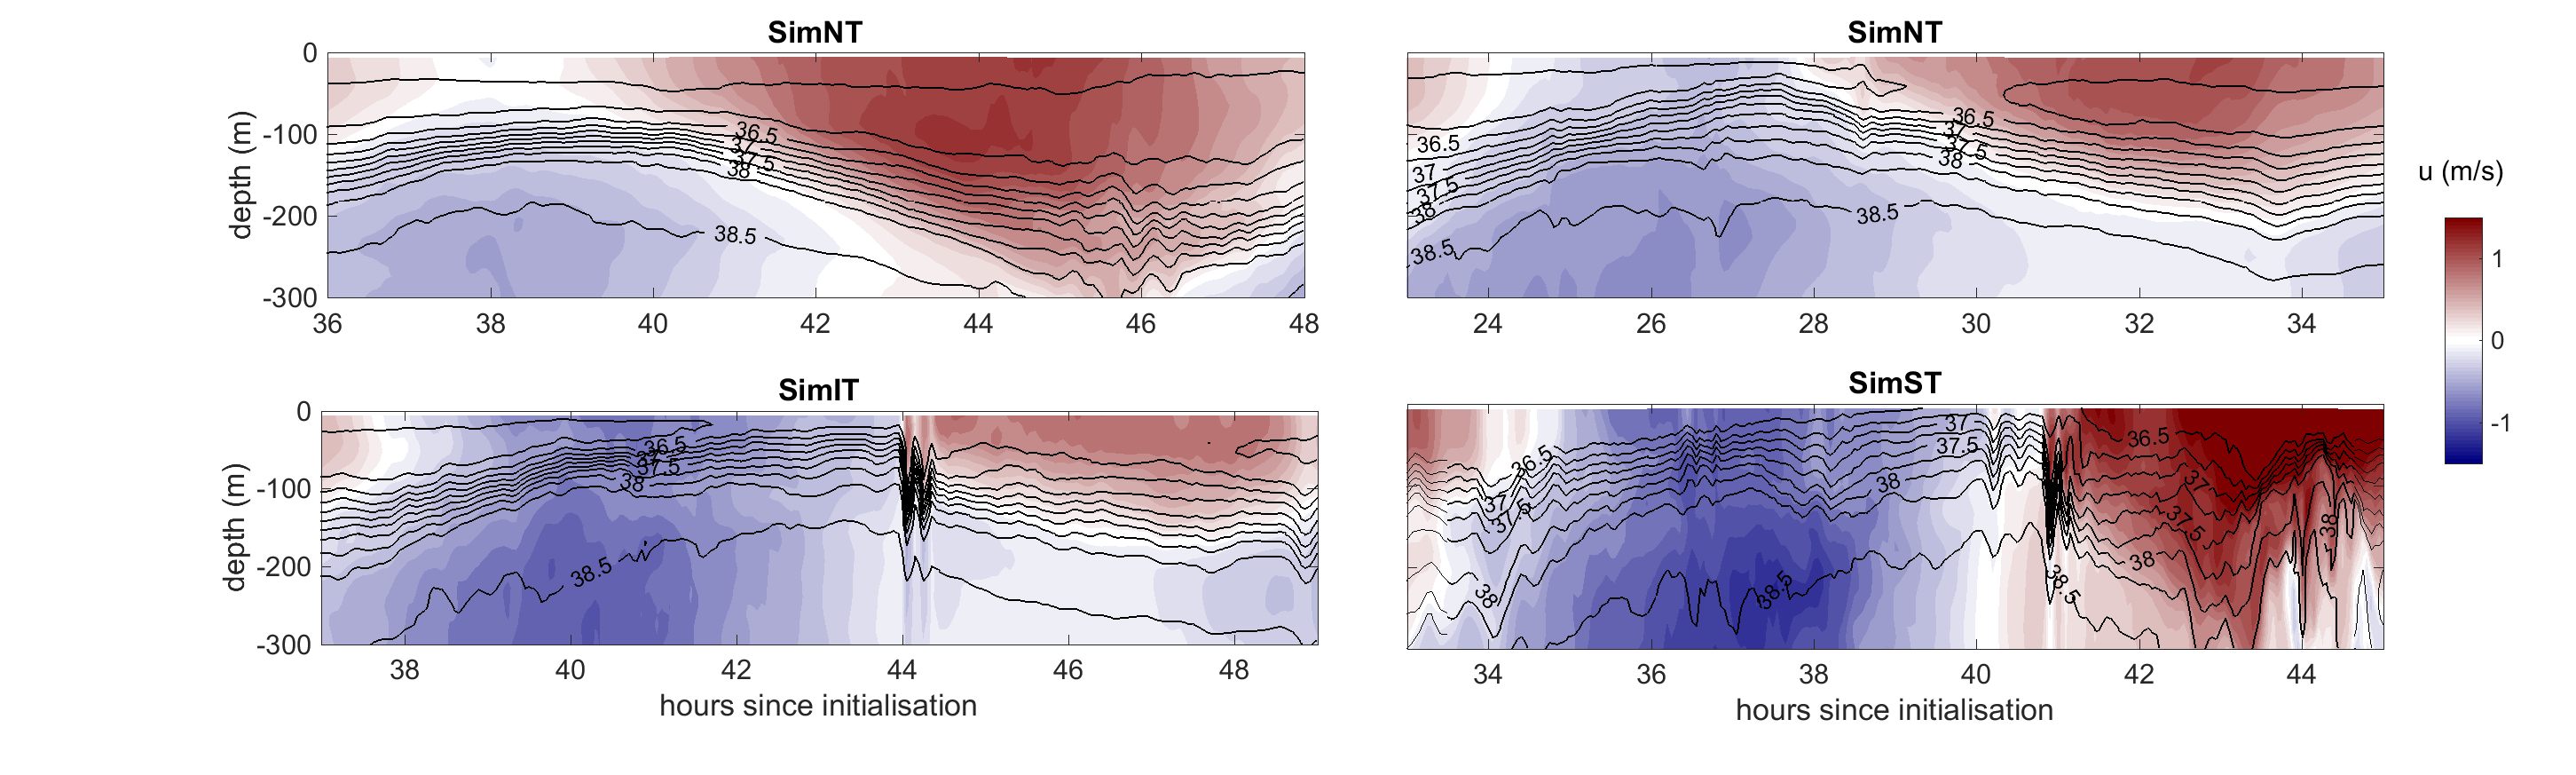
\includegraphics[width=\textwidth]{./GBR3D/US_M4SimMIV.png}
 \caption [Time series of salinity and zonal velocity in simulations SimNT, SimIT and SimST]{Time series of salinity (black lines) and zonal velocity (color) in the upper 300 m in simulations SimNT( A and B), SimIT (C) and SimST (D) of Section \noparref{sectionSim3D} at the gridpoint of coordinates (35.937°N;5.706°W). Abscises is simulation time. }
 \label{Fig_moor_USs}
\end{figure}

It is on the salinity interface observed at Mo5 mooring that the signal of propagating internal gravity waves can be spotted, sometimes matching with anomalies in the current field of mooring Mo4.

Figures \noparref{fig_moor_US1}.B3 at t = 3 h, \noparref{fig_moor_US2}.A3 at t = 8h30, and \noparref{fig_moor_US2}.B3 at t = 19h30, show as a recurring feature an abrupt lifting of the interface, that does not appear in the simulations data of Figure \noparref{Fig_moor_USs}.

Another recurring signal in Mo5-mooring data are the large amplitude troughs that can be seen during the inflow period of the tidal cycle. In this data set, it appears clearly in observation data made at t = 29 h in Figure \noparref{fig_moor_US2}.B3. In simulation data (for example t = 49 h in Figure \noparref{Fig_moor_USs}.C), this signal corresponds to a westward traveling train of ISWs that is generated by reflection off the Moroccan coast of the well-known eastward traveling ISWs train that is generated at CS.

The focus is now made on the signal showing up at Mo4 and Mo5 mooring, usually 3 hours or sooner after the maximal outflow at Mo2 mooring. Five distinctive types of signals are identified and categorized with letters o, L, B, S, and 2S :

\begin{itemize}
\item \underline{Linear-internal tide (o), Figures \noparref{fig_moor_US1}.A2-A3}: the depth of the salinity interface at Mo5 mooring and maximum shear at Mo4 mooring evolves linearly, except for some low amplitude traveling waves at the interface in Mo5 mooring at t = 10h30. At Mo2 mooring (Figure \noparref{fig_moor_US1}.a1), there is a distinctive shear in the water column during the preceding outflow, with slightly positive velocity in the upper layer. This signal is also seen in SimNT as shown in Figure \noparref{Fig_moor_USs}.A.
%
\item \underline{Small-amplitude internal wave (L), Figures \noparref{fig_moor_US1}.B2-B3}: in the salinity data, there is a signal that looks like two internal waves of relatively small amplitude (10 m) at Mo5 mooring at t = 4h30. At Mo4 mooring, the depth of maximum shear of zonal velocity still evolves in a linear manner as in the previous (o) case. At Mo2 mooring (Figure \noparref{fig_moor_US1}.A1), the interface of westward flow evolves at the same depth as in the (o) case but in the upper layer velocity becomes almost nil from t = 1 h to t = 3h30. This signal is also seen in SimNT in Figure \noparref{Fig_moor_USs}.B at t = 28.5 h of simulation, and is associated there in the velocity field with a mode-1 anomaly.
%
\item \underline{Internal-traveling bore (B), Figures \noparref{fig_moor_US2}.A2-A3}: at Mo5 mooring, the salinity interface drops by 50 m at t = 11 h which resembles the signal of a westward-propagating internal bore. At Mo4 mooring, however, the depth of maximum shear still evolves linearly, but before the arrival of the internal bore signal, the flow in the water column is negative at all depths. At Mo2 mooring over CS, the upper layer velocity is nil or lightly negative during the outflow. This type of signal is not recovered in the simulations that have been performed.
%
\item \underline{Train of internal-solitary waves (S), Figures \noparref{fig_moor_US2}.B2-B3}: a succession of seven troughs goes though Mo5 mooring starting at t = 24h15. The first one has an amplitude of 80 m. At Mo4 mooring, this series corresponds to mode-1 anomalies of the velocity field. At Mo2 mooring, the flow is westward throughout the water column during the preceding outflow, with an abrupt return to a sheared two-layer state at t = 22h30, corresponding to the loss of hydraulic control and the release of the western hydraulic jump over CS. In simulations, this type of signal is seen for instance in simIT and presented in Figure \noparref{Fig_moor_USs}.C with two troughs at  t = 44 h. In these simulations, this type of signal at mooring Mo4 and Mo5 follows the release of a s-jump type of hydraulic jump (i.e., at maximum outflow, the western hydraulic jump is located over the shallowest part of CS).
%
\item \underline{Two close trains of internal-solitary waves (2S), Figures \noparref{fig_moor_US3}.A1-A2}: five troughs can be seen propagating at Mo5 mooring starting at t = 2 h, but are not propagating in order of decreasing amplitude. The first trough has an amplitude of 80 m and is followed by two short-wavelength, small-amplitude troughs. Then at t = 2h30, an over-100-m amplitude trough propagates at Mo5 mooring. It is in turn followed by a smaller-amplitude trough. The mode-1 anomaly of the velocity field is seen clearly at Mo4 mooring for the first two waves, then the fourth larger amplitude one. At Mo2 mooring, as in the previous (S) case, the flow through the water column transitions from wholly westward to sheared two-layer at t = 1 h. In numerical simulation SimST (Figure \noparref{Fig_moor_USs}.D), four waves can be identified. They follow this pattern, the first two waves have decreasing amplitude, the third has a larger amplitude than the first two, and the fourth has a smaller amplitude. In this case, this pattern corresponds to two different trains of ISWs. The first (second) train corresponds to the previously  released hydraulic jump east (west) of CS. In the numerical simulations, this signal follows the release of a w-jump (i.e., at maximum outflow the west hydraulic jump is located over the western slope of CS).
\end{itemize}

Both S and 2S signals are linked to westward flow of the whole water column at CS, which should indicate that, as in the numerical simulations, a hydraulic jump was present west of Mo2 mooring.

The 2S case can be observed in numerical simulations and in Figure \noparref{Fig_moor_USs}.D. The amplitude of the first wave which corresponds to the eastern hydraulic jump of CS can however be very small. While the wave(s) produced by the release of the eastern hydraulic jump are always present, at the latitude of moorings Mo4 and Mo5, its amplitude depends (i) on the northern extent of the eastern hydraulic jump at maximum outflow (i.e., how high a latitude it reaches) and (ii) on the initial angle taken by the released non-linear wave as it first propagates in a slightly southern direction.

As the two sets of ISWs propagate further in the strait, the second train overtakes the first one. Indeed the propagation speed of ISWs depends on their amplitude (the larger the faster), so eventually they appear as a merged and sorted train of ISWs. For instance, the "S" structure in simulation appears because the wave released by the western hydraulic jump of CS overtook the eastern one(s) sooner due to their initial closeness.

So although it appears here that two cases are distinct (the S case following an s-jump and the 2S case following a w-jump), there might be a possibility that slowly propagating waves from an s-jump could also appear as a 2S structure at Mo4 and Mo5 mooring, and conclusion cannot be reached on the structure of the two hydraulic jumps at CS only on the basis of the signal at Mo4 and Mo5 moorings.


\subsection{Transition between outflow types \& ISWs generation in Gibraltar strait}

The classification of the previous section is applied to signals at Mo4 and Mo5 mooring following each outflow of the first observation period and is marked as annotations in Figure \noparref{fig_moor_US3}.B.

A pattern emerges linking outflow type and strength of the averaged currents at CS. The beginning of the period corresponds to the neap-tide part of the fortnightly cycle, and either (L) or (o) type of outflows are detected, with no hydraulic jump at CS. The first solitary wave is observed at Mo4 and Mo5 mooring the 12/10/2020. Due to the diurnal variation of the M2 tide, the tidal flow over the following period is weaker (less than 1 m/s) and the signal at Mo4 and Mo5 moorings is an (o) case.

Except for one specific (B) case (14/10/2020), during the remainder of the period, trains of ISWs (with either a S or 2S structure) are propagating through Mo4 and Mo5 mooring. The stronger outflows lead to (2S) signals in agreement with the numerical simulations presented in Section \noparref{sectionSim3D}. Under especially strong outflows, the internal hydraulic jump generated over CS is swept downstream as a w-jump, resulting in an initially increased distance between the eastern and western jumps. This distance may not be overcome as quickly upon release of the hydraulic jump as in the s-jump case. This explains the distinction between S and 2S cases, however as explained previously, for some outflows, the distinction between the two may remain subjective.

Only one (B) case is observed, it was not featured in numerical simulations so it is less evident whether it can be attributed to the presence of a hydraulic jump over CS. Whereas the variation with depth of currents at Mo2-mooring site in the preceding outflow shows a shallower interface and more westward currents in the upper layer than for the (o) and (L) cases, it may be more akin to a near supercritical flow regime engendering some form of propagating steepening interfacial disturbance.

It was seen in Section \noparref{section_sim3D_ISW} that, in numerical simulations, even if no hydraulic jump occurs at CS, the flow of the barotropic tide in the strait of Gibraltar can lead to the steepening of a long interfacial wave that later develops into a train of ISWs. This train contains a lesser number of ISWs than in the release of hydraulic jump case as it propagates toward the Alboran Sea. 

Figure \noparref{fig_SAROBS} is a SAR image taken during the Gibraltar 2020 campaign in the morning of October, 9. A curved surface signature of higher reflectivity can be seen in the Alboran Sea, looking like the front of an ISW (for example in Figure \noparref{fig_SARIES}.A). But looking at Figure \noparref{fig_moor_US3}.B, all preceding outflows are of the "L" case for the signal at Mo4 and Mo5 mooring at this date, with no hydraulic jump at CS. The small amplitude internal gravity wave that was observed at Mo5 mooring, if propagating east, could be responsible for the signal in the Alboran Sea that looks like a lone ISW, and is similar to what was encountered in simulations.

\begin{figure}[!h]
 \centering
 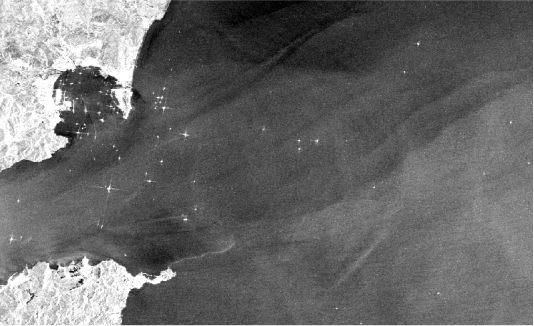
\includegraphics[width=0.6\textwidth]{./GBR3D/SAR_OBS_GEPETO.png}
 \caption [Sentinel-1 SAR image.]{Sentinel-1 Synthetic Aperture Radar (SAR) image from 09/10/2020 - 6h18am UTC.}
 \label{fig_SAROBS}
\end{figure}


\subsection{Discussion \& perspectives}

A first confrontation between numerical LES and observations has been carried out showing at least a qualitative agreement. Similarities are found between simulated fields and four of the five types of signals encountered in data of moorings Mo4 and Mo5. Two of those signals, namely "S" and "2S" structures have been shown to be trains of ISWs propagating after the release of the hydraulic jumps at Camarinal Sill. This release induces indeed a westward flow in the whole water column in Mo2 mooring data. 

Concerning the signal associated to "L" structures, the presence of the hydraulic jump is doubtful, but Figure \noparref{fig_SAROBS} provides a satellite image of what appears to be the signal of a lone large-amplitude internal wave propagating in the Alboran Sea after such an outflow. According to this observation, and in agreement with numerical simulations, the mechanism of release of the hydraulic jump might not be the only mechanism responsible for the generation of the observed ISWs in the strait of Gibraltar and in the western part of the Alboran sea. ISWs trains are indeed observed in other areas of the global ocean, without being linked to the establishment and to the release of a hydraulic jump (see for example \citet{chen_2017}).

Looking at the barotropic currents observed at the Mo2 mooring, there is a pattern linking the amplitude of the tide to the signal observed at the Mo4 and Mo5 moorings. Indeed there seems to be a threshold over which hydraulic jumps and solitary waves can be observed. The reproduction of this threshold in numerical simulations of the strait of Gibraltar is expected to be complex. Even in high-resolution regional modelling such as in Section \noparref{sectionSim3D}, the transition between regimes with or without hydraulic jumps depends greatly to the numerical configuration. The quality and realism of the simulated stratification, for example, play a crucial role in controlling the "criticality" of the atlantic-mediterranean exchange flow and consequently in setting the date of appearance of the hydraulic jump. The quality of the water masses simulated numerically can obviously depend greatly on the quality of the atmospheric and large-scale forcing, knowing that the former has been neglected in the present configurations. Other important physical factors are the high-sensitivity to the quality of the high-resolution bathymetric data and to the tidal forcing.

Several improvements shall be made in a future study and \color{red}are already been (????non?????)\color{black} evaluated: 
\begin{itemize}
\item Atmospheric fluxes are specified at the surface of the ocean.  This provides a better representation of the stratification in the upper surface and has important consequences on the characteristics of the pycnocline and thus on the characteristics of the internal waves, bores and solitons.
\item The high-resolution dynamics in the strait of Gibraltar can now be explicitly simulated by downscaling the regional circulation (from the Gulf of Cadix to midway of the Alboran Sea). A three-step embedding has already been carried out using AGRIF library from 900-m to 60-m resolution simulations through a 180-m resolution implementation.
\end{itemize}
 
 \color{red}
\section{Appendix : Interface determination between Atlantic and Mediterranean waters}
\label{appendix_interface}

The choice is made to analyze the flow in the Strait of Gibraltar as a two-layer exchange flow based on salinity. 

To determine this salinity, first profiles of salinity in the three simulations are fitted to hyperbolic tangent formulations following \citet{sannino_2007}. However, contrary to \citet{sannino_2007} that used this definition to consider the interface as a distinct third layer of finite thickness with its own dynamic, here only the median value of the hyperbolic tangent profile is taken as salinity of the interface between Atlantic and Mediterranean waters. 

%The salinity value attributed to the interface however could evolve in the Strait. In a first step, profiles of salinity in the three simulations are fitted to hyperbolic tangent formulations following \citet{sannino_2007} that used this fitted profile to define an interface layer of finite thickness. However, contrary to \citet{sannino_2007} that used this definition to consider the interface as a distinct third layer in the flow, here only the median value of the hyperbolic tangent profile is taken as salinity of the interface delineating between Atlantic and Mediterranean waters.

Profiles are analyzed for all three simulations at sections of constant longitude and for various timesteps in the tidal cycle, thus giving both time and spacial variation in this salinity value.

However, the choice is made to only retain a longitudinal variation for the definition of the interfacial salinity and so for each longitudinal section in each simulation, a value is averaged in time and latitude that is presented in Figure \noparref{fig_defintf}. On this figure is also plotted the finally chosen expression for the value of the salinity interface in the Strait of Gibraltar that reflects the asymmetry of water mass composition with respect to Camarinal Sill:
\begin{equation}
	S_I(l)=tanh(\frac{l-L_{CS}}{dl})\frac{S_M-S_m}{2}+\frac{S_M+S_m}{2}
	\label{eqSinterfaceApp}
\end{equation}
with $L_{CS}=5.75^o$, $dl=0.25^o$, the location and width of the Camarinal Sill in degrees, $S_M=37.39$ and $S_m=37.1$ the max and minimum interface values taken respectively east and west of the sill.

\begin{figure}[!h]
 \centering
 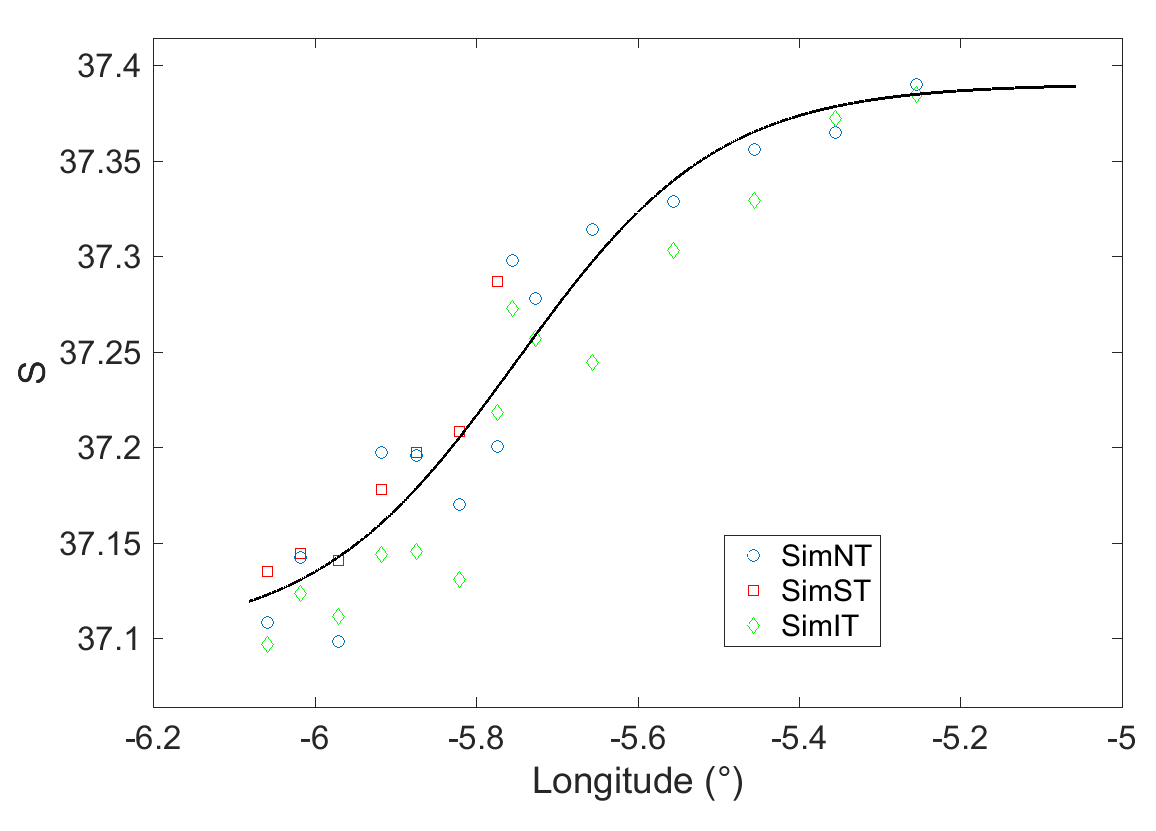
\includegraphics[width=0.6\textwidth]{./GBR3D/salinite_interface_papier.png}
 \caption [Value of salinity of the interface between Atlantic and Mediterranean waters]{Value of salinity of the interface between Atlantic and Mediterranean waters from either average of the median values of fitted hyperbolic tangent profiles in simulations SimNT (blue circles), SimIT (green diamonds) and SimST (red squares) at various longitude, or the curve of equation $S_I(l)$ (black line, see text).}
 \label{fig_defintf}
\end{figure}

This definition is applied online in simulation to define the Atlantic and Mediterranean layers, compute average velocity and Froude number, and reduce variables outputs.
\color{black}

\section{Appendix : Singular Value Decomposition (SVD)}
\label{annexeSVD}
Incomplete Singular Value Decomposition (SVD) consists in finding a basis of $k$\footnote{In an incomplete decomposition, $k$ the number of singular values on which to decompose A can be specified.} singular values and orthonormal singular vectors for a matrix A (complex or real), so that :
\begin{equation}
A = U \Sigma V^* 
\end{equation}
If A has dimensions G x T, $U$ is a G x $k$ matrix, while $V$ (and its conjugate $V^*$) is a k x T matrix. $U$ and $V$ are called the left and right singular vectors respectively, and $\Sigma$ is the diagonal $k$ x $k$ matrix of singular values associated to each couple of singular vectors.

To analyze a time-varying signal of a variable $\psi$ on a 3D grid of G grid points, the spatial field of each of the T time-steps is appended into one column of length G to create the GxT matrix A, where T are the number of iterations of the 3D field. 

After proceeding with the SVD of this matrix A, the 3D spatial structure of the $i^{th}$ left-singular vector is recomputed together with its time-evolution ($i^{th}$ right-singular vector).

In Section \noparref{sectionSim2D}, SVD is applied to the complex field $\psi=w+i\ u$. %consecutive vectors of the basis with close singular value and that exhibited similar time-variations were combined to ... .
In Section \noparref{sectionSim3D}, SVD is applied to the field of the real quantity $Q$.
